%!TEX root = Thesis_main.tex

\addcontentsline{toc}{chapter}{Appendices}
\section{Super Mega Bot Datasheet}
\label{AppA}

\begin{figure}[h]
	\begin{center} 
		\subfigure[Supermegabot]{
		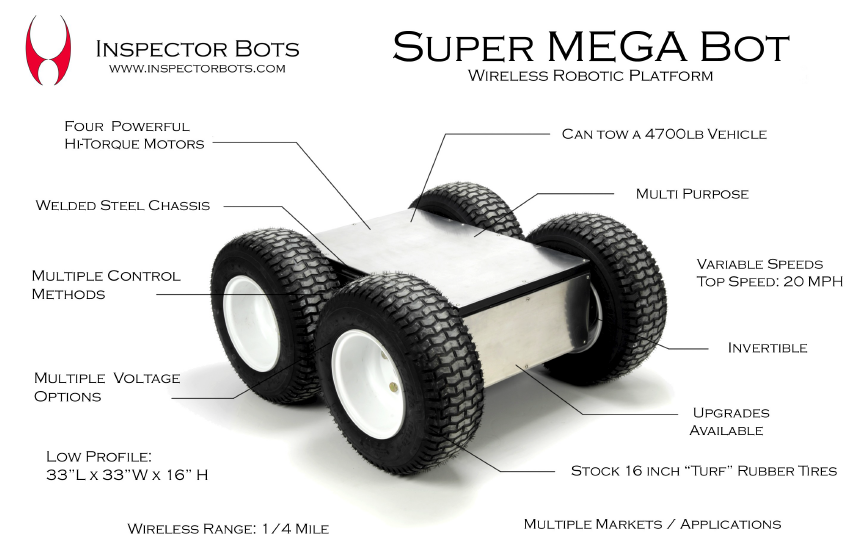
\includegraphics[scale=0.43]{SuperMegaBot}
		\centering
		\label{fig:SuperMegaBot}}
		\qquad
		\subfigure[Wiring scheme]{
		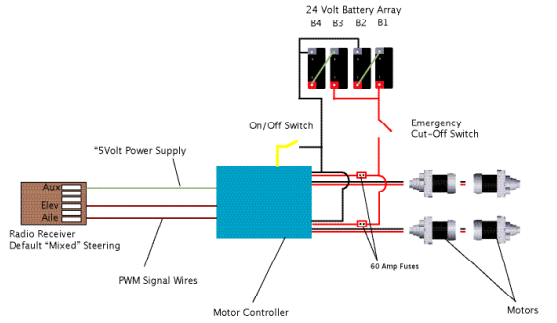
\includegraphics[scale=0.43]{SMBwires}
		\centering
		\label{SMB Wiring}}
	\end{center}
\end{figure}
Its base model comes with:\\
•	Chassis: Powder Coated Steel and Aluminum \\
•	Dimensions: 84cm L x 84cm W x 40.64cm H, Weight: 109 kg\\
•	Drive: Four Electric Motors\\
•	Load Capacity: 113,5 kg\\
•	Speed Controllers: RoboteQ 2x VDC2450\\
•	Speed: 0-16 km/h \\
•	Suspension: Rigid\\
•	Tires: Interchangeable, Pneumatic, 40.64cm Diameter Turf Tires\\
\url{https://www.youtube.com/watch?v=3X8IWnR1QDI}
